\subsection {Sprint 3}

A \textit{sprint} 3 foi o momento onde houve maior foco em questões de usabilidade e experiência do usuário. Nessa \textit{sprint} houve a participação do time de \textit{design} do Lab Livre para auxiliar na definição dos elementos visuais e na organização do fluxo de uso da ferramenta. Em geral, os requisitos da \textit{sprint} foram definidos como:

\begin{itemize}
	\item \textbf{Requisito 1 da Sprint 3}: Adequar os componentes visuais da tela de visualização e edição do texto de acordo com o protótipo elaborado pelo time de \textit{design};
	\item \textbf{Requisito 2 da Sprint 3}: Ajustar o fluxo de uso da funcionalidade de acordo com a jornada mapeada pelo time de produto.
\end{itemize}

\subsubsection {Requisito 1 da Sprint 3}

Na Figura \ref{fig:prototipo-rascunho-figma}, pode-se conferir uma captura de tela do protótipo criado pelo time de \textit{design} na ferramenta Figma. Com intuito de preservar o nível de desempenho obtido pela refatoração realizada na \textit{sprint} 1, as modificações visuais foram majoritariamente feitas através do uso de CSS, com pouquíssima alteração no HTML.

\begin{figure}[htbp]
  \centering
  \caption{Protótipo da tela de rascunho}
  \label{fig:prototipo-rascunho-figma}
  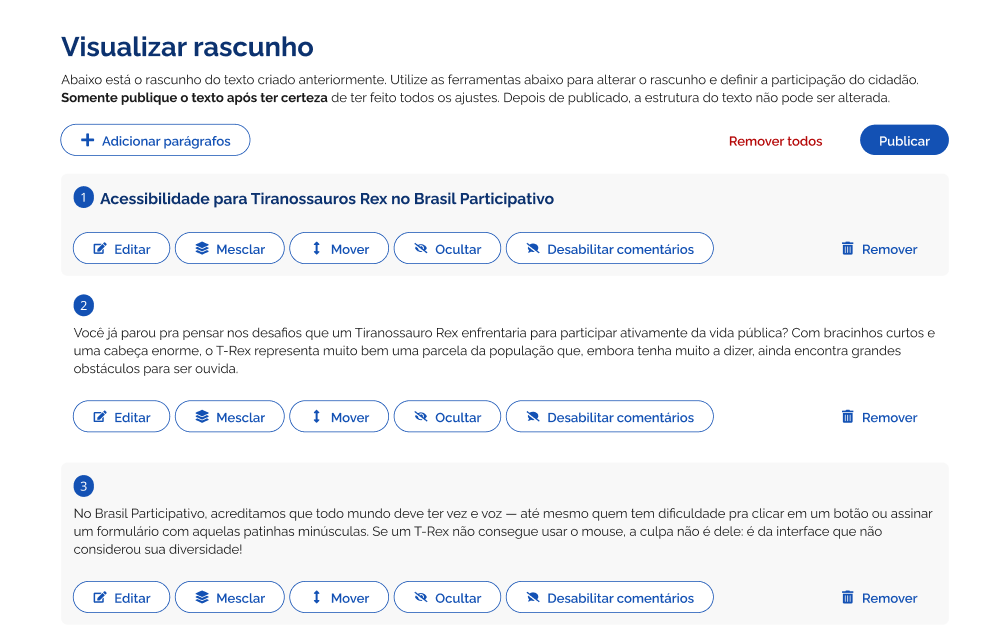
\includegraphics[width=\textwidth]{figuras/prototipo-rascunho-figma.png}
  \fonte{Time de \textit{design} do Lab Livre - UnB}
\end{figure}

A estilização foi feita principalmente através de regras aplicadas a classes HTML utilizando o \textit{Syntactically Awesome Style Sheets} (SASS), uma linguagem de extensão para CSS. As regras de estilo foram codificadas no arquivo \texttt{participatory-text.scss}.

Para utilizar da estilização por classes, na própria \textit{partial} \texttt{\_lightweight\_text\_render}, para cada parágrafo a ser renderizado, é instanciado um \texttt{Array} para guardar quais classes HTML são aplicáveis naquele contexto. Para isso, são feitas verificações sobre o tipo, visibilidade e estado do parágrafo, além de checar se a \textit{partial} está sendo renderizada no modo edição ou visualização. Na Figura \ref{fig:estilizacao-classes-partial} é demonstrado de forma resumida o código utilizado.

\begin{figure}[htbp]
  \centering
  \caption{Exemplo código fonte para estilização dinâmica com classes}
  \label{fig:estilizacao-classes-partial}
  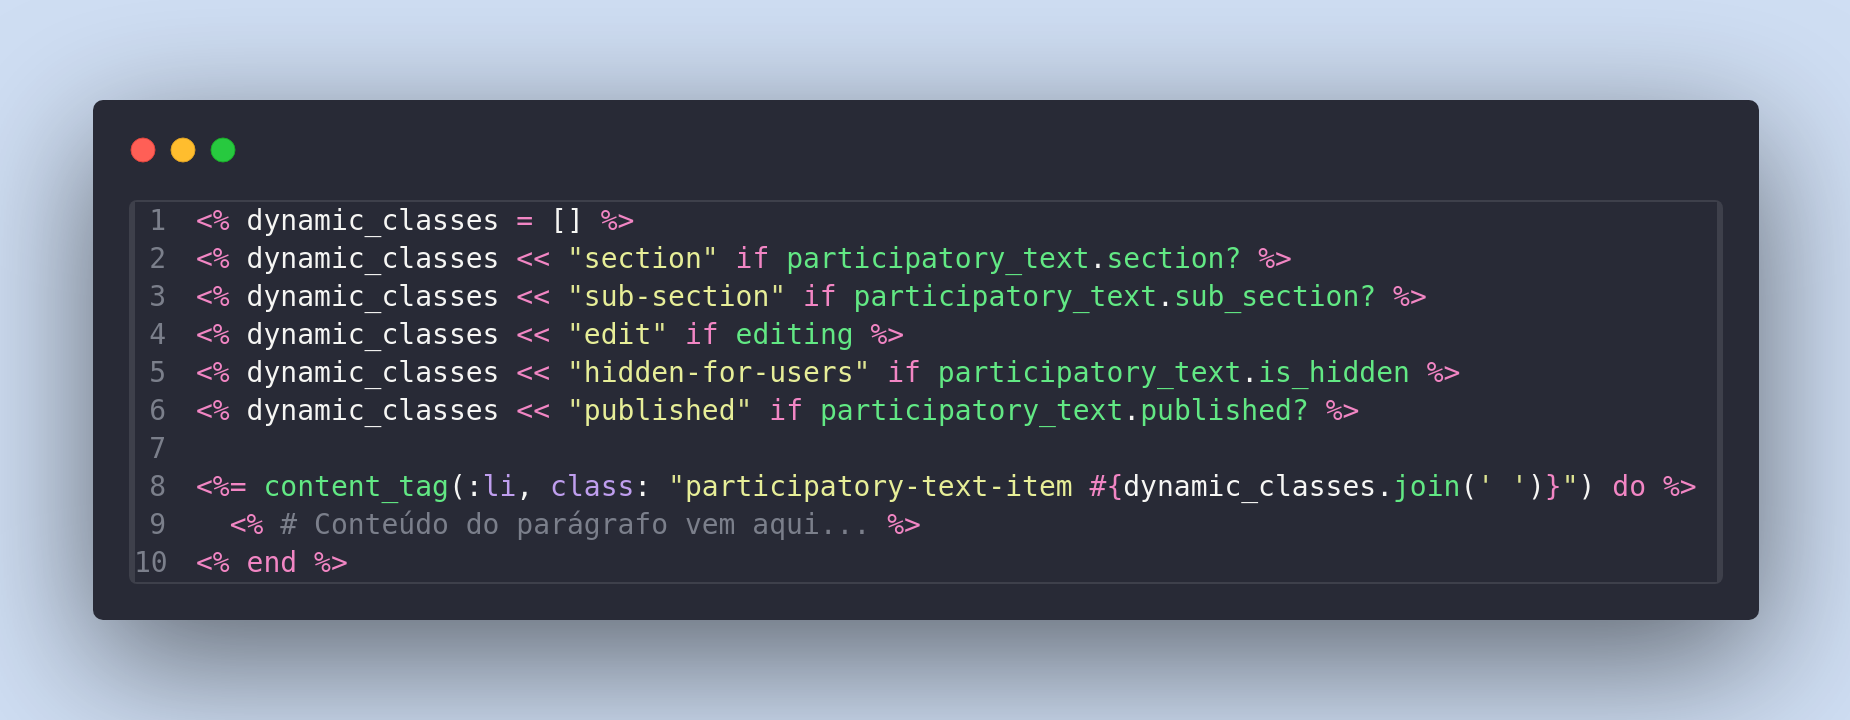
\includegraphics[width=\textwidth]{figuras/estilizacao-classes-partial.png}
  \fonte{Próprio autor}
\end{figure}

Com essa abordagem, foram adicionadas apenas verificações com \textit{if/else} para dinamicamente alterar as classes do elemento \texttt{<li>} que envolve o conteúdo do parágrafo.
Essa estratégia evita o uso desnecessário de \textit{partials}, que poderia trazer novamente gargalos de desempenho para a \textit{view}, e evita também duplicação de código, algo que as \textit{partials} se propõe a resolver.

Um comparativo do antes e depois do visual da tela de edição do texto pode ser conferido através das figuras: Figura \ref{fig:editar-texto-visual-antes}, que mostra o estado anterior às modificações, e Figura \ref{fig:editar-texto-visual-depois} que mostra o estado após as modificações.

\begin{figure}[htbp]
  \centering
  \caption{Tela de edição de textos antes da adequação visual}
  \label{fig:editar-texto-visual-antes}
  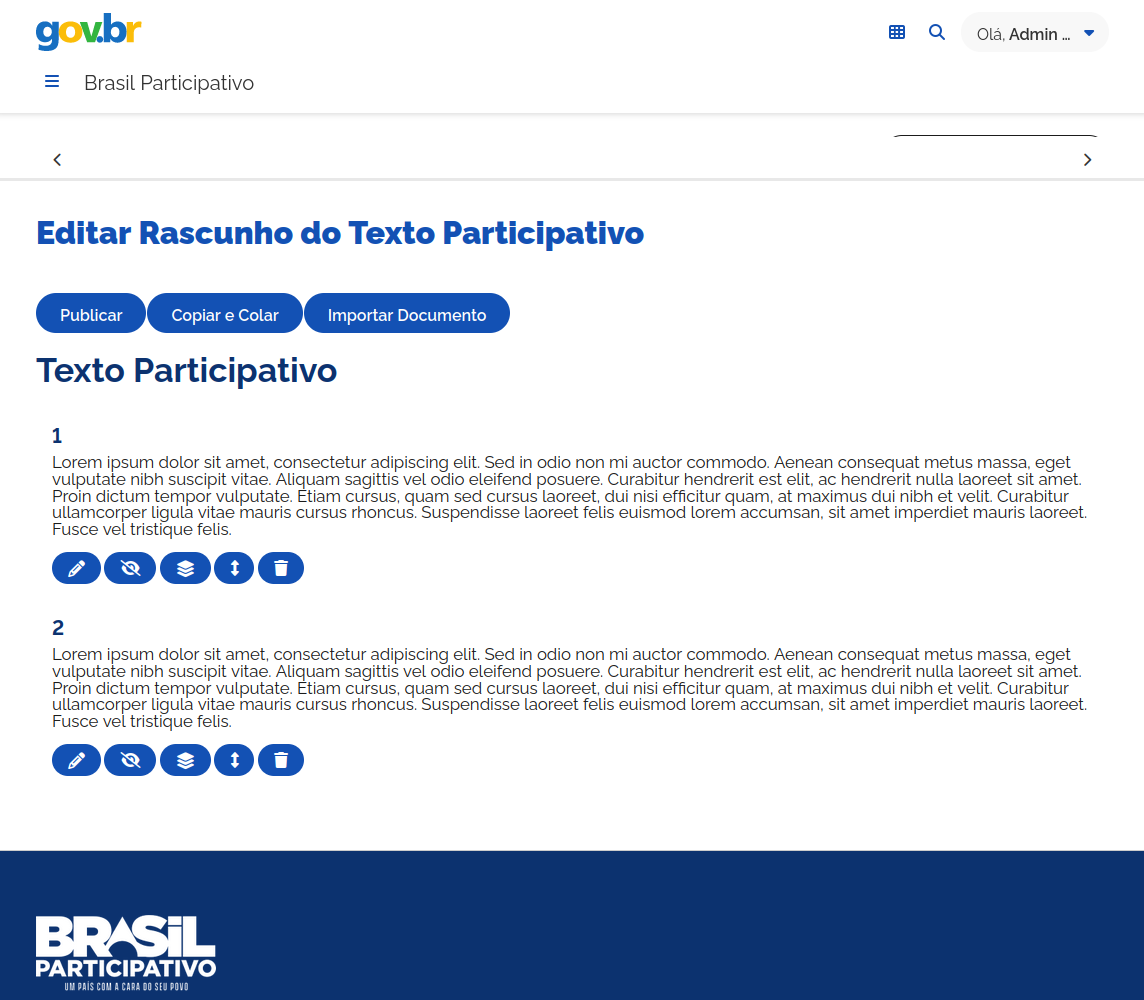
\includegraphics[width=\textwidth]{figuras/editar-texto-visual-antes.png}
  \fonte{Próprio autor}
\end{figure}

\begin{figure}[htbp]
  \centering
  \caption{Tela de edição de textos depois da adequação visual}
  \label{fig:editar-texto-visual-depois}
  
\includegraphics[width=\textwidth]{figuras/editar-texto-visual-depois.png}
  \fonte{Próprio autor}
\end{figure}

\subsubsection {Requisito 2 da Sprint 3}

O fluxo de uso da ferramenta de textos participativos ainda possuia sobreposições com a versão anterior à adequação da página de edição do texto. Por conta da tela de edição estar junta da tela de visualização do texto no contexto \texttt{public}, várias transições ocorriam entre contexto \texttt{admin} para contexto \texttt{public}, que são visualmente diferentes, durante a jornada de uso da funcionalidade.
Para que o usuário administrador acessasse a página de edição do texto, era preciso primeiramente navegar pela página do componente no painel \textit{admin}, para só então clicar em um botão para o redirecionar para a tela desejada.

Sendo assim, foram realizados ajustes para que o usuário seja direcionado diretamente para páginas que façam sentido para o estado atual do texto participativo. Essas modificações foram feitas apenas com o uso de redirecionamentos nas \textit{controllers} com o uso do método \texttt{redirect\_to}.
Dessa forma, esse ajuste não teve impacto no requisito de desempenho, dado que bastava fazer uma verificação sobre o estado do texto participativo e realizar ou não o \textit{redirect} para outra página.

O trabalho realizado na \textit{sprint} também contou com a participação do time de desenvolvimento do Lab Livre. As alterações podem ser conferidas na íntegra nos \textit{Merge Requests}:

\begin{enumerate}
  \item \url{https://gitlab.com/lappis-unb/decidimbr/decidim-govbr/-/merge_requests/603}
  \item \url{https://gitlab.com/lappis-unb/decidimbr/decidim-govbr/-/merge_requests/612}
  \item \url{https://gitlab.com/lappis-unb/decidimbr/decidim-govbr/-/merge_requests/613}
  \item \url{https://gitlab.com/lappis-unb/decidimbr/decidim-govbr/-/merge_requests/615}
  \item \url{https://gitlab.com/lappis-unb/decidimbr/decidim-govbr/-/merge_requests/628}
\end{enumerate}
